\section{Detector sensitivity}
\label{sec:sim}
%%%%%%%%%%%%%%%%%%%%%%%%%%%%%%%%%%%%%%%%%%%%%%%%%%%%%%%%%%%%%%%%%%%%%%%%%%%%%%%%%%%%%%%%%%%%%%%%%%%%%%%%%%%%%%%%%%%%%%%%
The sensitivity of the detector is estimated by its ability to identify an anisotropic component in the scintillation photons emission pattern (signal), over the isotropic one (background). The photon emission pattern is modeled using a combination of isotropic emission and one or two beams:
\begin{equation}
\mathcal{F}(\theta,\phi) = (1-r_{aniso}) \cdot f_{iso} + r_{aniso}\cdot\left[r_1 f_G(\sigma_1) + r_2 f_G(\sigma_2) \right], 
\end{equation}  
where  $f_{iso}$ is the PDF of an isotropic emission, $f_G$ is a PDF of a Gaussian distribution with half width $\sigma$. $r_{aniso}$ is the anisotropic emission fraction, and $r_{1,2}$ are the relative beams intensities. The first beam direction is random, and the second's is either random 
(''uncorrelated``) or opposite to the first's (''correlated``). The different emission patterns used here are summarized in Table~\ref{tab:AnisoPattern}.
 
\begin{table}[h]
  \centering
  \caption{Anisotropic emission patterns. For all patterns $r_{aniso}$ = 0.1}
  \label{tab:AnisoPattern}
  \begin{tabular}{|c |c |c|cc|cc|c|}
  \hline
  Pattern no. & No. of beams & type & \multicolumn{2}{c|}{Beam half widths}& \multicolumn{2}{c|}{Signal fractions} & $N^{'}$ \\
 % \hline
  &              &      &  $\sigma_1$ & $\sigma_2$   &  $r_1$ & $r_2$ &   \\
  \hline
  1 & 1 & single beam & $5^{0}$ & - & 1 & 0 & 3200\\
  %\hline
   2 & 1 & single beam & $15^{0}$ & - & 1 & 0 & 4630\\
  %\hline
   3 & 2 & correlated & $5^{0}$ & $5^{0}$ & 0.5 & 0.5 &  4520  \\
  %\hline
   4 & 2 & correlated & $15^{0}$ & $15^{0}$ & 0.5 & 0.5 & 9770  \\
  %\hline
   5 & 2 & uncorrelated & $5^{0}$ & $5^{0}$ & 0.5 & 0.5 & 9370\\
  %\hline
   6 & 2 & uncorrelated & $5^{0}$ & $10^{0}$ & 0.5 & 0.5 & 19500\\
  %\hline
   7 & 2 & uncorrelated & $15^{0}$ & $15^{0}$ & 0.5 & 0.5 & 28200\\
  %\hline
   8 & 2 & uncorrelated & $10^{0}$ & $30^{0}$ & 0.5 & 0.5 & 49900\\
  %\hline
   9 & 2 & uncorrelated & $10^{0}$ & $30^{0}$ & 0.2 & 0.8 & 56000\\
  %\hline
    10 & 2 & uncorrelated & $30^{0}$ & $10^{0}$ & 0.2 & 0.8 & 43000\\
  \hline
 \end{tabular}
\end{table} 
 
 

A GEANT4 based simulation is used to model the detector system, generate photons, propagate them through the detector, and obtain a PMT hit pattern. The photons detected at the 
PMTs are mapped and put through a statistical test to check the detector's sensitivity towards the different emission patterns.

The relevant geometrical and optical parameters, which are used in the simulation, are listed in Table~\ref{tab:OptPar}. 
The scintillation light produced in a particular 
event is emitted by a cloud of excimers. This cloud is assumed to have a linear size much smaller than that 
of the optical system. Therefore each event is simulated as a number of photons that are emitted from a point 
in the LXe with some emission pattern (see Table~\ref{tab:AnisoPattern}). The number of generated photons for each event is taken to be Poisson(50), which correspond to an energy deposition of $\sim2.5\mathrm{keV}$  or $\sim7\mathrm{keV}$ for ER or NR respectively. The LXe target is much smaller than the mean free path of the source particles, and to 
account for that the events are uniformly generated in the LXe volume.
The probability for a photon being transmitted/reflected at a given surface is 
determined by Fresnel's equations, which include Snell's law for the transmitted light, 
and specular reflection for the reflected light. The boundary surfaces between different media
such as, the LXe--HPFS, HPFS--vacuum and vacuum--PMT, are assumed to be perfectly smooth, 
therefore enabling only specular reflection. 
The photons reaching the PMTs can either be detected, absorbed or reflected from the photocathode 
or PMT window. A simplified approach of the above possibilities is considered:
a photon reaching the PMT has a 30\% probability to be detected (since the PMTs have QE $\geq$ 30\%), 
50\% probability to get absorbed and 20\% probability to get specularly reflected. 

%%%%%%%%%%%%%%%%%%%%%%%%%%%%%%%%%%%%%%%%%%%%%%%%%%%%%%%%%%%%%%%%%%%%%%%%%%%%%%%%%%%%%%%
\begin{table}[h]
  \centering
  \caption{The parameters used in simulation}
  \label{tab:OptPar}
  \begin{tabular}{|l c||l c|}
  \hline
  Parameter & Value & Parameter & Value \\
  \hline
  LXe absorption length & 100 cm & HPFS shell inner radius & 1cm \\
  %\hline
  LXe scattering length & 35 cm & HPFS shell thickness & 2 cm\\
  %\hline
  LXe refractive index & 1.61  & PMT QE &  30\% \\
 % \hline
  LXe Scintillation wavelength & 178& PMT distance from center & 39 mm\\
 % \hline
  HPFS absorption length & 100 cm  & Number of PMT & 20 \\
  %\hline
  HPFS refractive index & 1.57 & PMT active area & 22mm $\times$ 22mm \\
  HPFS scattering length & $\infty$ & Invar tube diameter & 1 mm\\
  \hline
 \end{tabular}
\end{table}
%%%%%%%%%%%%%%%%%%%%%%%%%%%%%%%%%%%%%%%%%%%%%%%%%%%%%%%%%%%%%%%%%%%%%%%%%%%%%%%%%%%%%%%


The statistical fluctuation 
in the electronic signal generated in a PMT for a certain number of incident photon is 
taken into account. The R8520 PMTs have 20\% probability 
for double photoelectric emission for 178 nm photons, which is included in the simulation.
Each detected photon on a PMT is assigned a uniformly random position on the PMT surface. 
The direction of this point with respect 
to the center of the LXe sphere is defined as the incident direction of the photon. The direction information 
is then used to calculate the angles between all possible pairs of photon for any event and 
calculate the correlation between all angle pairs. \RanComment{Do you want to add fig of correlations iso and aniso?} 
\mmd{Good idea. Iso and a few choses aniso are fine?}

In order to quantify the anisotropicity of the emission, 
the angle correlation distribution of an anisotropic hit pattern is compared to that of the isotropic 
pattern. A $\chi^2$ test statistics is used where the reduced $\chi^2$ is defined as: 

\begin{equation}
\chi^2_\nu = \frac{1}{\nu} \sum^{\nu}_{i=1} \frac{(O_i - E_i)^2}{E_i},
\label{redchi2}
\end{equation}

where $E_i$ is the expected number of entries for an isotropic emission obtained from a sample of $10^5$ simulated events. 
$O_i$ is the observed number of entries, and $\nu$ is the total number of angle correlation bins 
which is also the degree of freedom. Sixty bins of identical width are used.


To asses the needed exposure to claim discovery assuming one of the   pattern mentioned above, $10^4$ data sets are generated and tested against the null hypothesis. This is repeated for increasing number of events between $1-4000$ assuming different values of the anisotropy fraction ($r_{aniso}$). The <$\chi^2_\nu$> 
and its 2$\sigma$ band for pattern 1, assuming $r_{aniso} =0.1$ overlaid with the corresponding values  for an isotropic emission are shown in Fig.~\ref{fig:pattern1}.  
The values of $N^{'}$, required to claim $5\sigma$ discovery, for different values of $r_{aniso}$ are calculated for each pattern as illustrated in Fig.~\ref{fig:convergence}.
The number of events 
$N^{'}$ for $r_{aniso} =0.1$ are summarized in Table~\ref{tab:AnisoPattern} for all emission patterns.

A simulation with two typical sources that emit isotropically, a 10 $\mu$Ci $^{137}Cs$ (662\,keV gamma), and a 2.7 $\mu$Ci AmBe ( 5\,MeV neutron), shows that for an average yield of 
50photons/event,  the rate of events in the detector is: $1.25\times10^{4}$\,events/day for NR and 625\,events/day for ER. 
Therefore a system that can operate stably for few weeks 
is expected to do reasonable measurements for ER and NR events.


%%%%%%%%%%%%%%%%%%%%%%%%%%%%%%%%%%%%%%%%%%%%%%%%%%%%%%%%%%%%%%%%%%%%%%%%%
\begin{figure}[h]
\centerline{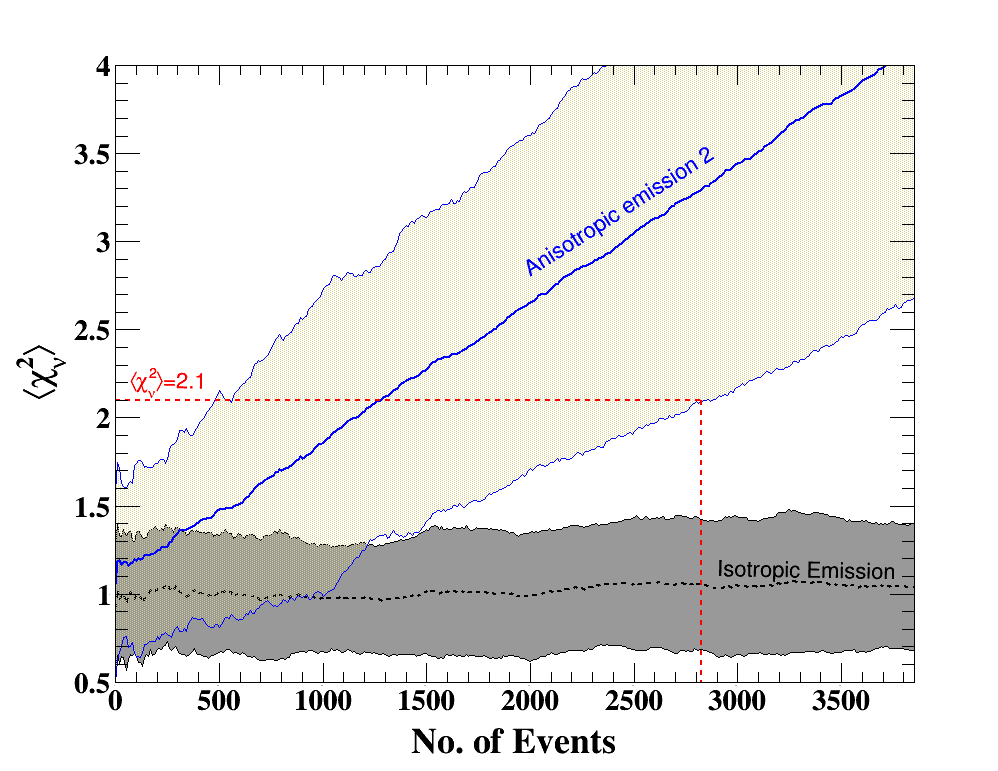
\includegraphics[width=0.5\linewidth]{Pattern1.png}}
\caption{<$\chi^2_\nu$> and its $2\sigma$ band for isotropic emission (black) and for pattern 2 (blue). The <$\chi^2_\nu$> for 
isotropic emission fluctuate around 1 with $\sigma$ = 0.2 which is consistent with 
the expected value of $\frac{1}{\sqrt{30}} \equiv 0.18$ for reduced $\chi^2$ distribution 
with 60 degrees of freedom. $\sim3000$ events are needed to claim  5$\sigma$ discovery ($\chi^2_\nu=2.1$) for this emission pattern}
\label{fig:pattern1}
\end{figure}
%%%%%%%%%%%%%%%%%%%%%%%%%%%%%%%%%%%%%%%%%%%%%%%%%%%%%%%%%%%%%%%%%%%%%%%%%%%%

%%%%%%%%%%%%%%%%%%%%%%%%%%%%%%%%%%%%%%%%%%%%%%%%%%%%%%%%%%%%%%%%%%%%%%%%%
\begin{figure}[h]
\centering
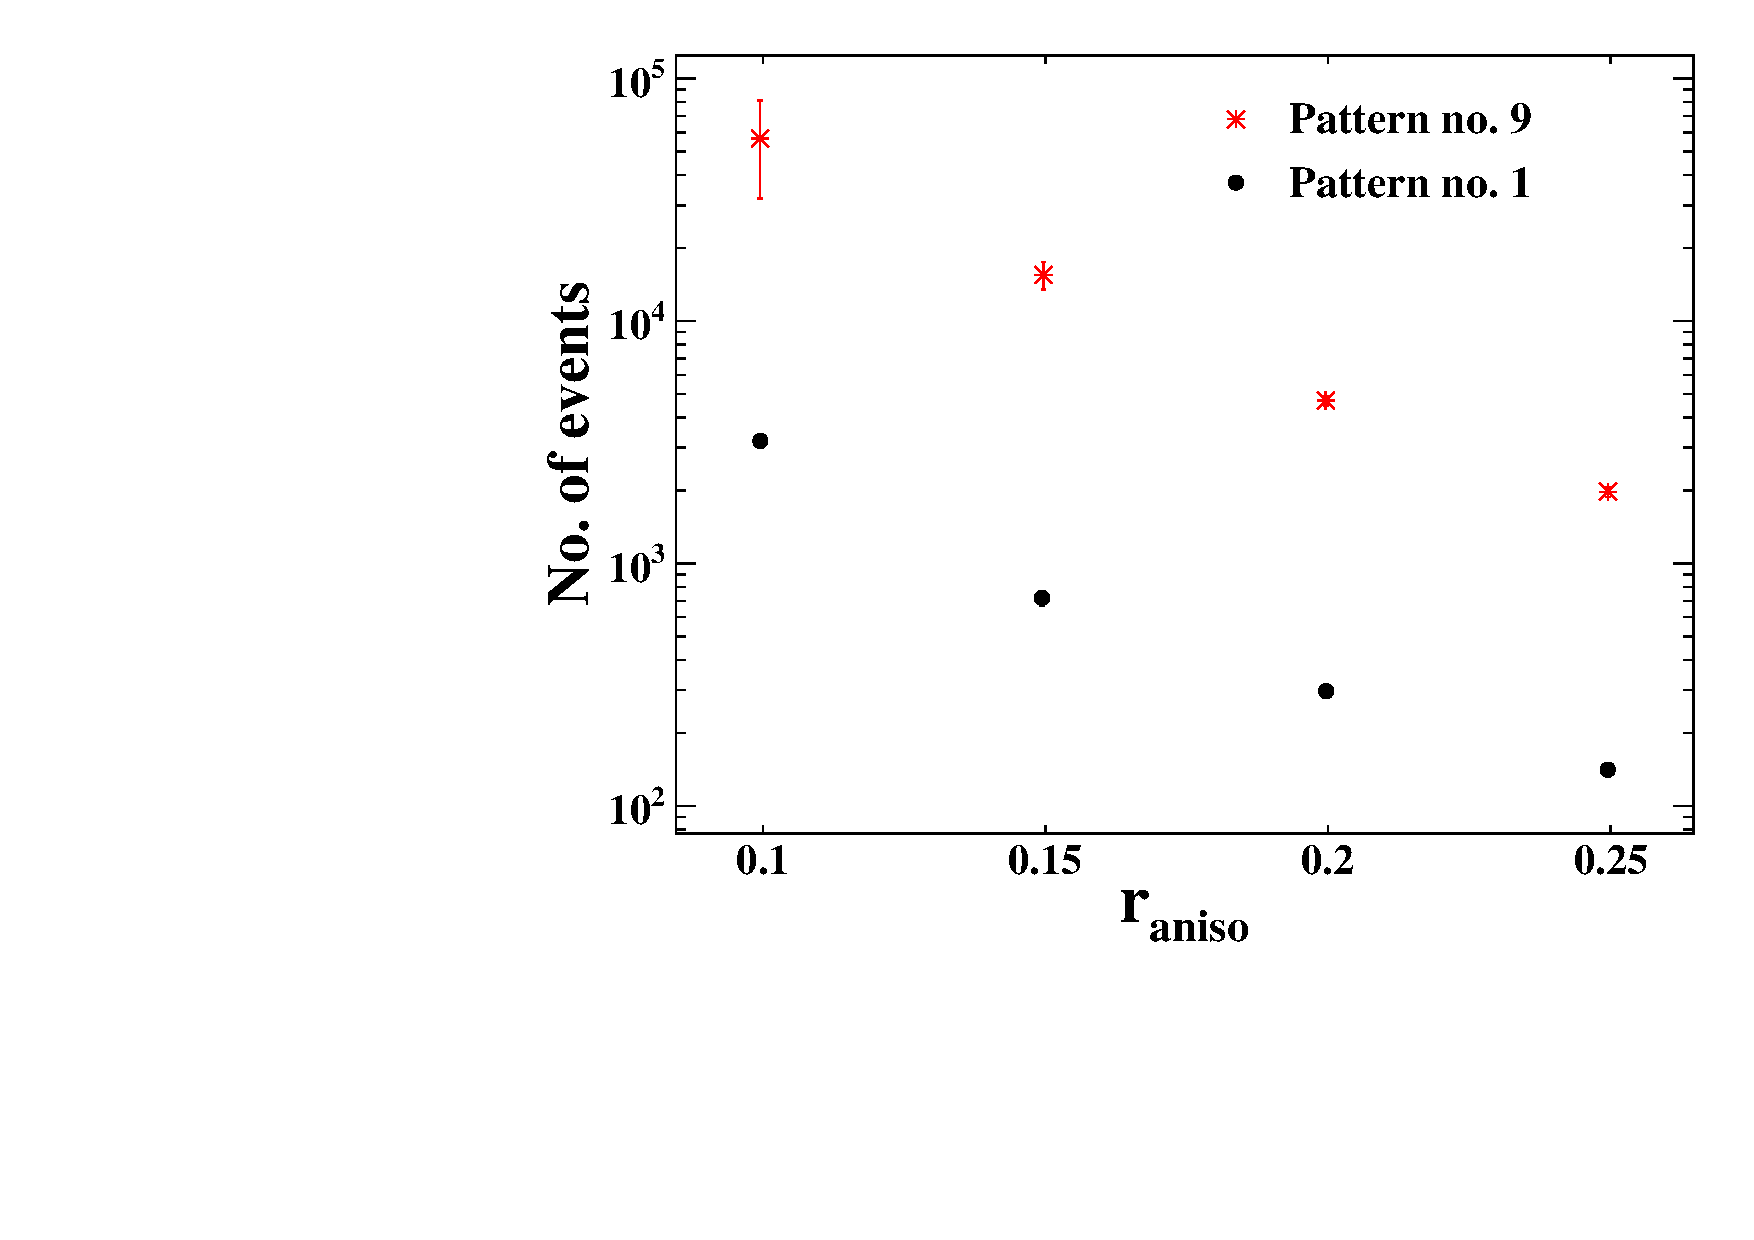
\includegraphics[width=0.45\linewidth]{ConvergenceVsRaniso.pdf}
\caption{The number of events needed for each emission pattern to achieve $5\sigma$ presented only for pattern 1 and 9. Here 
$r_{aniso}$ = 0.1. for four different values of $r_{aniso}$.}
\label{fig:convergence}
\end{figure}
%%%%%%%%%%%%%%%%%%%%%%%%%%%%%%%%%%%%%%%%%%%%%%%%%%%%%%%%%%%%%%%%%%%%%%%%%%%%


